\section{Agregacja zbioru danych - wyniki}

Na początku działania algorytmu agent jest inicjalizowany w identyczny sposób jak w metodzie \textit{klonowania zachowań}, na zestawie trajektorii \textit{świadomie prezentującego eksperta} o wielkości 6000 kroków. Następnie agent odbywa 3 iteracje metody agregowania zbioru danych. Każda iteracja to odegranie jednego epizodu o długości 2000 kroków, podczas których ekspert może w dowolnym momencie przejąć kontrolę nad agentem i poprawić jego zachowanie. Kroki wykonane przez eksperta są dodawane do \textit{pamięci powtórek} 5 razy w celu zwiększenia wagi decyzji eksperta. Po zakończeniu każdego epizodu wagi sieci neuronowej są resetowane, a cała sieć jest uczona od początku na podstawie rozszerzonego zestawu danych (tzn. na podstawie początkowych trajektorii uczących i kroków wykonanych podczas gry przez eksperta). Po nauczeniu sieci wykonywanych jest 20 epizodów testowych.

Przejęcie kontroli nad agentem odbywa się poprzez wciśnięcie klawisza \textit{p}. Po przejęciu kontroli środowisko przechodzi w synchroniczny tryb gry, każdorazowo czekając na następny ruch gracza. Ekspert kontrolujący agenta może przy użyciu dedykowanych klawiszy wykonywać dowolną kombinację ruchów, a po zakończeniu prezentacji oddać kontrolę agentowi ponownie używając klawisza \textit{p}.

Testy zostały przeprowadzone wyłącznie na scenariuszu \textit{Trudne zbieranie apteczek}, ponieważ zachowanie agenta w scenariuszu \textit{Obrona środka} nie przejawiało żadnych wyraźnych błędów, za pomocą poprawy których można było by osiągnąć poprawę w stosunku do wyników metody \textit{klonowania zachowań} z zestawem trajektorii \textit{świadomie prezentującego eksperta}.

Eksperyment został powtórzony 10 razy. Już po tej niewielkiej liczbie powtórzeń tendencja zachowania wynikowego agenta i osiąganych przez niego wyników była wyraźna, dlatego dalsze czasochłonne eksperymenty nie były kontynuowane. Testy z wykorzystaniem pozostałych technik przekazywania kontroli do eksperta nie zostały przeprowadzone, ponieważ zastosowanie innej metody nie wyeliminowałoby problemów badanego algorytmu.

\subsection {Zachowanie eksperta}
Ekspert skupia się na wyeliminowaniu problemu wchodzenia w miny. Ekspert przejmuje kontrolę gdy agent zachowuje się, jakby miał popełnić błąd. Ekspert sporadycznie reaguje na nieoptymalne, ale nie błędne zachowanie agenta. Wielokrotnie ekspert nie potrafi zareagować na działanie agenta wystarczająco szybko, żeby uniknąć popełnienia błędu. Ponieważ ekspert zawsze przejmuje kontrolę w sytuacjach awaryjnych, jego zachowania mogą być odmienne od zachowań, które przejawiałby w identycznej sytuacji podczas normalnej gry. W szczególności ekspert:

\begin{itemize}
\item{znajdując się przed miną nie wymija jej, ale w miarę możliwości odwraca się i szuka innej drogi}
\item{jeżeli agent zapętli się na niewielkim fragmencie labiryntu skierowuje go do innych rejonów}
\item{pomaga wychodzić z krótkich pętli zachowań (np. zablokowanie w rogu) w optymalnym kierunku}
\item{sporadycznie nakierowuje agenta na konkretne apteczki, jeżeli w danej sytuacji jego polityka wyboru apteczek jest błędna}
\item{wielokrotnie przejmuje kontrolę nad agentem zbyt późno, żeby zapobiec wejściu w minę}
\end{itemize}


\subsection{Wyniki}\label{dagger_results}
W tabeli \ref{tab:dagger_results} i na rysunku \ref{fig:dagger_results} przedstawiono średnie wyniki uzyskiwane przez metodę \textit{agregacji zbioru danych} podczas eksperymentów. Punktem startowym są wyniki uzyskane za pomocą metody \textit{klonowania zachowań}, bez dodatkowych działań eksperta. W kolejnych wierszach tabeli przedstawione są średnie wyniki testów w kolejnych epizodach nauki. Ocenione kroki oznaczają orientacyjną liczbę kroków, które ocenił ekspert (wliczając to początkowe trajektorie uczące). Obejrzane kroki to liczba kroków wykonanych podczas nauki (wliczając to początkowe trajektorie uczące i kroki agenta, które obserwował ekspert). Zmiana wyniku i odchylenie standardowe wyniku oznaczają średnią i odchylenie standardowe zmiany wyniku testowego w stosunku do wyników testowych sprzed 1 epizodu. 

Uczenie sieci na podstawie 6000 kroków trajektorii trwa około minuty, podobnie jak wykonanie 20 gier testowych. Każdy epizod gry agenta trwa około dwie minuty, ponieważ przejęcie kontroli nad agentem i decydowanie o optymalnym ruchu dla danego stanu jest w praktyce wolniejsze niż normalna, płynna gra. W sumie każda iteracja metody \textit{agregacji zbioru danych} trwa około 4 minut.

\begin{figure}[H]
		\ffigbox{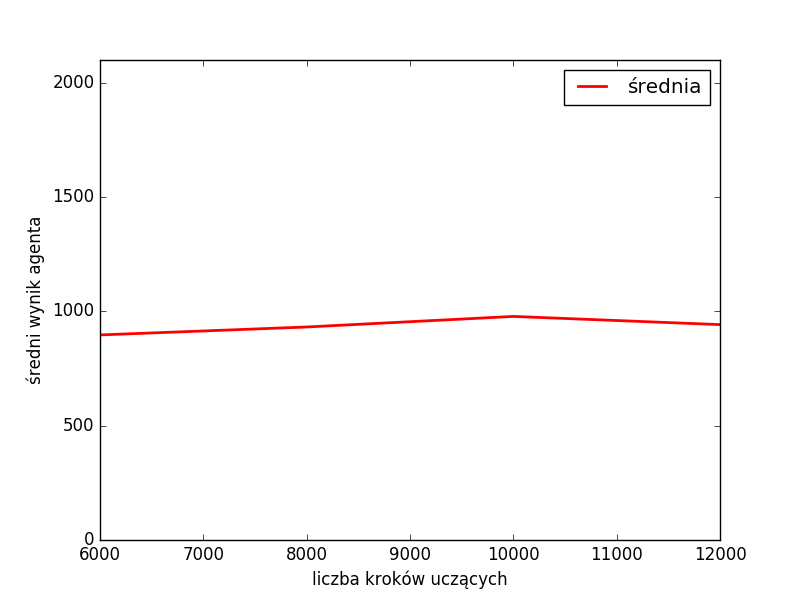
\includegraphics[scale = 0.7]{figures/figures/results/da_hg_plot.png}}{\caption{Wyniki agenta nauczonego za pomocą metody \textit{agregacji zbioru danych} w zależności od liczby kroków uczących w scenariuszu \textit{Trudne zbieranie apteczek}}\label{fig:dagger_results}}
\end{figure}

\begin{figure}[H]
\csvautotabular{data/dagger_results.csv}{\caption{Wyniki agenta nauczonego za pomocą metody \textit{agregacji zbioru danych} w zależności od liczby kroków uczących w scenariuszu \textit{Trudne zbieranie apteczek}.}\label{tab:dagger_results}}
\end{figure}

\subsection {Zachowanie agenta}
Dla istotnej części powtórzeń eksperymentu wizualna ocena zachowania agenta jest odwrotna od oceny wynikającej ze zmiany wyników. Już po pierwszym epizodzie zaczynają się pojawiać objawy przeuczenia: agent często ,,wpada w rezonans'' na rozwidleniach i w rogach labiryntu (na zmianę wykonuje akcje ,,lewo'' i ,,prawo'' bez ruszania się z miejsca), w stopniu znacznie większym niż w metodzie bazowej, oraz wielokrotnie utyka w jednym, małym obszarze labiryntu (np. wybiera na każdym rozwidleniu skręt w prawo i wraca po chwili do punktu wyjścia).

Chwilami można zaobserwować częściowe omijanie min, najczęściej jednak ten sam agent po kilku wzorowych ominięciach min wchodzi bez zawahania prosto w następną. Zdarza się też, że agent postawiony przed miną, przy braku jakichkolwiek apteczek w polu widzenia po chwili ,,rezonującego'' wahania wchodzi z premedytacją prosto w tę minę. Po zakończeniu uczenia agent regularnie zacina się w losowych miejscach labiryntu, co nie zdarza się raczej na początku uczenia.

Kolejne iteracje metody w średnim przypadku prowadzą do zwiększenia wyników agenta, jednakże wzrost wyników w stosunku do przejrzanej liczby klatek wypada znacznie gorzej niż wzrost wyników metody \textit{kopiowania zachowań} przy takim samym zwiększeniu liczby klatek. Jeszcze gorzej wypada porównanie wzrostu wyników w stosunku do czasu trwania algorytmu. 

\subsection {Analiza i wnioski}

Ekspert przejmuje kontrolę w tylko w sytuacjach awaryjnych, a jego decyzje muszą być dołączone do zbioru danych z większą wagą, żeby wywarły jakikolwiek wpływ na zachowanie agenta. Z pierwszego powodu zachowanie eksperta podczas iteracji metody może zasadniczo różnić się od zachowania które ekspert przejawiałby znajdując się w analogicznej sytuacji podczas normalnej, ciągłej gry.

Przy tak małym zestawie danych uczących zachowania niespójne z początkowymi trajektoriami uczącymi sprawiają, że agent silnie generalizuje ,,poprawki'' eksperta, co pogarsza jego zachowanie w sytuacjach, w których zachowywał się wcześniej poprawnie. W praktyce metoda rozdmuchuje problemy \textit{ klonowania zachowań}, które miała eliminować.

Proces nauki jest długi i znacznie bardziej obciążający dla eksperta niż zbieranie trajektorii, z przeplatającymi się momentami oczekiwania na zakończenie przetwarzania i momentami skupionej kontroli zachowań agenta - dlatego czas trwania całego algorytmu, a nie kroki wykonane podczas nauki przez agenta powinny być przedmiotem porównania. Z punktu widzenia eksperta poświęcenie tego samego czasu na generowanie kolejnych trajektorii prezentacyjnych jest znacznie mniej obciążające niż obserwowanie agenta i rozważanie w każdym momencie, czy agent jest na skraju popełnienia błędu i konieczna jest reakcja.

Średni wynik uzyskiwany przez agenta w kolejnych iteracjach metody rośnie, ale wzrost wyników jest wolniejszy niż przy nauce z pomocą innej metody przy analogicznym zwiększaniu liczby kroków uczących. Znaczny rozrzut wyników sprawia też, że \textit{agregację zbioru danych} trudno uznać za solidną.
